 \begin{surferIntroPage}{Dünya Rekoru Yüzeyler}{record_chmutovoktic}{Dünya Rekoru Yüzeyler}
Eğer bir yüzeyin üstünde bir sivrilik varsa o yüzeye \emph{tekil} denir; aksi takdirde yüzeye \emph{düzgün, yumuşak} denir. Sivrilik noktalarına \emph{tekillik} denir. Düzgün yüzeylere örnek, küre ya da simittir (torus); bunları görmek için aşağıdaki ilk iki resme bakın.
Rastgele bir yüzey seçerseniz  neredeyse her zaman düzgün bir yüzeyle karşılaşacaksınız.
 \begin{center}
      \vspace{-0.2cm}
      \begin{tabular}{@{}c@{}c@{}c@{\quad}c@{}c@{}c@{}c@{}}
        \begin{tabular}{@{}c@{}}
          düzgün:
        \end{tabular}
        &
        \begin{tabular}{@{}c@{}}
          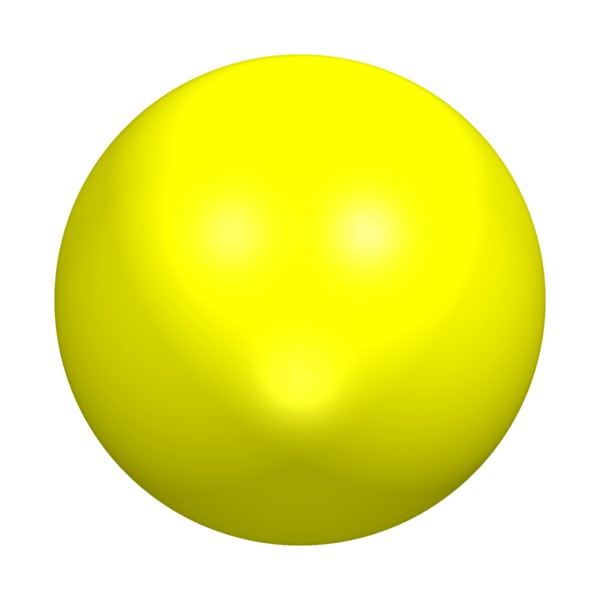
\includegraphics[width=1.1cm]{kugel}
        \end{tabular}
        &
        \begin{tabular}{@{}c@{}}
          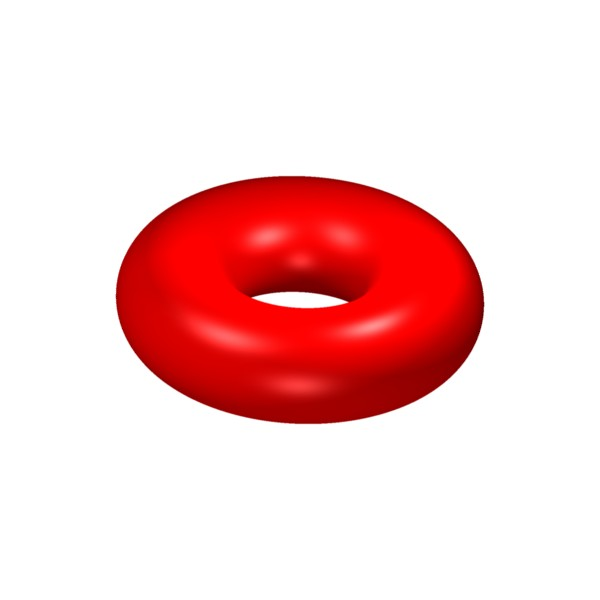
\includegraphics[width=1.1cm]{torus}
        \end{tabular}
        &
        \begin{tabular}{@{}c@{}}
          çok\\
          tekillikli:
        \end{tabular}
        &
        \begin{tabular}{c@{}@{}}
          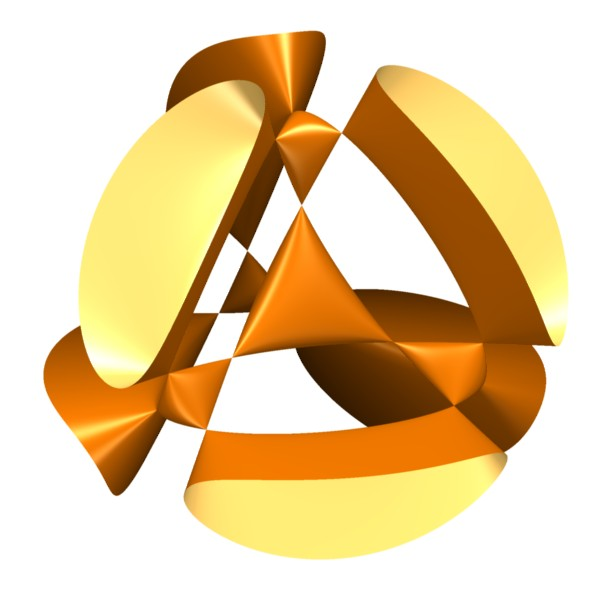
\includegraphics[width=1.1cm]{kummer}
        \end{tabular}
        &
        \begin{tabular}{c@{}@{}}
          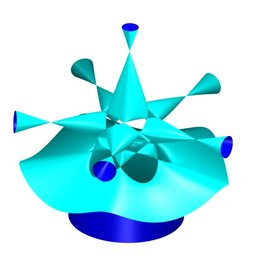
\includegraphics[width=1.1cm]{togliatti}
        \end{tabular}
        &
        \begin{tabular}{c@{}@{}}
          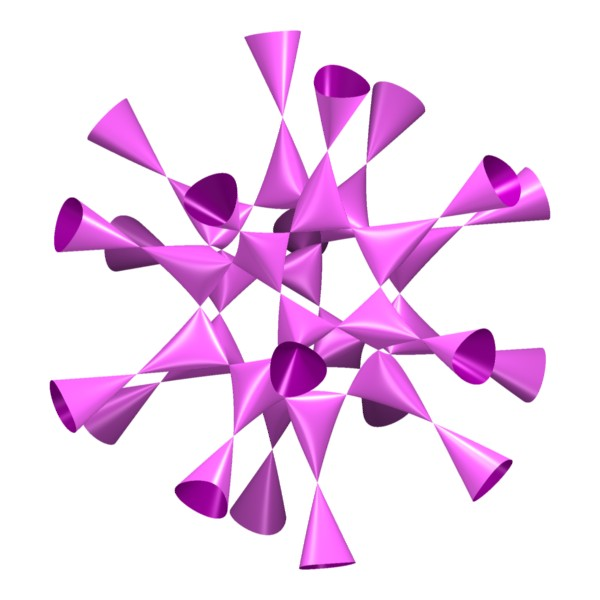
\includegraphics[width=1.1cm]{barth_sextic}
        \end{tabular}
      \end{tabular}
    \end{center}
    \vspace{-0.2cm}
Dolayısıyla bir yüzeyin tekilliklere sahip olması çok özel bir durumdur. Bu yüzden tekillikler bir yüzeyin en ilginç noktalarıdır. SURFER yazılımında yüzeyler polinomlar aracılığıyla tanımlanır; yani değişkenlerin üsleri sıfırdan büyükeşittir.
Bir polinomda en büyük üsse polinomun derecesi denir. Matematikte araştırma sorularından biri, belirli bir dereceli yüzeyin kaç tane tekilliğe sahip olabileceğidir. Bir polinomun derecesini $d$ ile, 
olası en fazla tekillik sayısını da  $\mu(d)$ ile göstereceğiz.

Bu  $\mu(d)$  sayısını hesaplamak epey zor. $d=1,2,3,4$ gibi küçük dereceler için  $\mu(d)$ 
$19.$ yüzyıldan beri biliniyor. $d=5$ için ancak 1980'de, $d=6$ içinse daha 1996'da belirlenebildi.  
Derecesi 7 olan bir polinom için olası en fazla tekillik sayısı hala bilinmiyor.
Bu problemi tamamen halletmek daha çok zaman alacak gibi görünüyor. \\  Bilinen birkaç sonuç şöyle:
    
   \begin{center}
      \begin{tabular}{r|cccccccc|c}
        $d$ & $1$ & $2$ & $3$ & $4$ & $5$ & $6$ & $7$ & $8$ & $d$\\
        \hline
        \hline
        \rule{0pt}{1.2em}$\mu(d)\ge$ & $0$ & $1$ & $4$ & $16$ & $31$ & $65$ &
        $99$ & $168$ & 
        $\approx \frac{5}{12}d^3$\\[0.3em]
        \hline
        \rule{0pt}{1.2em}$\mu(d)\le$ & $0$ & $1$ & $4$ & $16$ & $31$ & $65$ &
        $104$ & $174$ & $\approx \frac{4}{9}d^3$
      \end{tabular}
    \end{center}
\end{surferIntroPage}
